\documentclass[11pt,a4paper]{amsart}
\usepackage[margin=1in]{geometry}
\usepackage{amsmath,amssymb,amsthm,mathtools}
\usepackage[expansion=false]{microtype}
\usepackage{tikz}
\usepackage[colorlinks=true,linkcolor=black,citecolor=black,urlcolor=black]{hyperref}
\usepackage[nameinlink,capitalize]{cleveref}
\hypersetup{
 pdftitle={Coframe rigidity and finite stationary separation for skew Schur functions},
 pdfauthor={John Shields},
 pdfkeywords={skew Schur function, Jacobi--Trudi coframe, fixed-cap rigidity, finite stationary identity, unit restoration, boundary reconstruction, determinant}}
\pdfinfo{/ORCID (https://orcid.org/0009-0004-3882-4571)}
\numberwithin{equation}{section}
\theoremstyle{plain}
\newtheorem{theorem}{Theorem}[section]
\newtheorem{proposition}[theorem]{Proposition}
\newtheorem{lemma}[theorem]{Lemma}
\newtheorem{corollary}[theorem]{Corollary}
\theoremstyle{definition}
\newtheorem{definition}[theorem]{Definition}
\newtheorem{remark}[theorem]{Remark}
\newtheorem{example}[theorem]{Example}
\newcommand{\Q}{\mathbb Q}
\newcommand{\JT}{\operatorname{JT}}
\newcommand{\ord}{\operatorname{ord}}
\newcommand{\Row}{\operatorname{Row}}

\title[Coframe rigidity and stationary separation]
{Coframe rigidity and finite stationary separation\\for skew Schur functions}
\author{John Shields}
\date{October 22, 2026}
\thanks{Independent researcher, Ginza 2-15-2, KR Ginza II 5F, Chuo-ku, Tokyo, Japan 104-0061.\\
\hspace*{\parindent}Corresponding author: \href{mailto:math@johnnyshields.com}{math@johnnyshields.com}.  ORCID: \href{https://orcid.org/0009-0004-3882-4571}{0009-0004-3882-4571}.}
\subjclass[2020]{Primary 05E05; Secondary 15A15}
\keywords{skew Schur function, Jacobi--Trudi coframe, fixed-cap rigidity,
finite stationary identity, unit restoration, boundary reconstruction, determinant}

\begin{document}
\begin{abstract}
The skew Schur function of a connected diagram, together with the function
obtained by splicing the same fixed connected cap to it, determines the
diagram up to translation.  We prove this using complete rational
Jacobi--Trudi coframes, retaining every unit and inverse pole.  For
zero-free diagrams and caps, a separate linearized theorem detects every
nonzero constant-weight combination of vacancy restorations from the two
observations.  These results imply finite stationary separation: a
shifted positive-power identity with a fixed rational potential forces
two equal-function connected diagrams to coincide.  Its precision is
fixed by the supplied span and includes the terminal coefficient.
We also treat a whole moving potential by field descent and prove an
unshifted exclusion for opposite ends of one diagram.  A weak-cap theorem
recovers absolute flags, including units, from the complete rational
coframe.
\end{abstract}
\maketitle

\section{Introduction}\label{sec:introduction}

A skew Schur function need not determine a connected skew diagram up to
translation or rotation \cite{Reiner2007Coincidences}.  Even rotation can
hide boundary data needed for reconstruction: the two hooks
\((2,1)\) and \((2,2)/(1)\) have the same function but different full beta
lists.  The question here is which complete rational boundary observations
restore that information.

A Jacobi--Trudi coframe records the entire solution of a boundary-column
system.  Its support remembers the native columns, and its product with
the complete-generator series remembers the native rows.  Entries of
index zero belong to both lists and remain in the matrix.  Deleting them
before solving changes the rational observation, even when a leading
homogeneous determinant is unchanged.

For connected diagrams \(B,K\), the \(00\)-splice
\(K\mathbin{\triangleleft}B\) joins their full boundary lists at a position
occupied by neither internal word.  Its precise lists are
\eqref{sc:splice-flags}.  Our fixed-cap theorem, \Cref{sc:fixed-cap}, says
that
\[
 B\longmapsto (s_B,s_{K\triangleleft B})
\]
is injective on connected normalized diagrams for each fixed literal
connected \(K\).  The same cap must be used on both sides; equality of cap
functions is not the hypothesis.  \Cref{fig:cell-splice} illustrates the
operation on the equal hook pair.

Nonlinear injectivity does not imply injectivity of a linearization.
For a zero-free diagram, a vacancy is an internal beta position absent
from both lists.  Restoring its row and column produces a bordered
determinant.  \Cref{sc:linearized-cap} proves independently that the whole
child and same-cap variations detect every nonzero combination of these
restorations with constant rational weights, provided both child and cap
are zero-free.  The rational weights allowed in the native-equation
calculation of \Cref{sc:unit-expansion} are a different contract.

The finite stationary theorem uses the clipped alternating operator
\(\mathcal T_{G,C}\) defined in \eqref{sc:finite-operator}.  For complete
coframes of actual connected diagrams with equal whole functions,
\Cref{sc:positive-power} proves that
\[
 \mathcal T_{G,C}(zH^p)+z\mathcal T_{G,C}(H)r(H)
                  =0\pmod{z^{2M}},\qquad p\ge2,
\]
forces literal equality.  Here \(M\) is the supplied span and \(r\) is a
fixed rational function over a field independent of the positive raw
letters.  The clock is transcendental over that field.  The coefficient
of degree \(2M-1\) is part of the hypothesis; the equal hooks in
\Cref{ex:terminal-coframes} show how the potential can first occur there.
\Cref{cor:stationary-field-descent} allows a potential in a larger neutral
field when a whole moving homomorphism is supplied.  Every dependent
coordinate and inverse entry moves under that map.

The opposite-end equation in \Cref{ph:unshifted-exclusion} is unshifted
and concerns one diagram and its rotation.  It is not the preceding
theorem with the initial \(z\) canceled.  Finite clipping contributes the
whole cap polynomial in \eqref{sc:exact-shift-cap}.  Its proof retains
connected and disconnected proper corners, genuine units, and the
exponent-two endpoint exceptions.

Connected skew-Schur irreducibility is used in its corrected form due to
Barekat, Reiner, and van Willigenburg
\cite{Barekat2009CoincidencesCorrigendum}; overlap and shape invariants are
from \cite{Reiner2007Coincidences}.  The two-boundary reconstruction results
of \cite{Shields2026SkewSchur} use first-row deletion and overlap-one row
extension.  The present \(00\)-splice instead replaces the top beta when
the cap is a row, and is not that extension.

\Cref{sec:coframe-coordinates} establishes the full-flag coordinates,
coframe atlas, defect bounds, and weak-cap reconstruction.
\Cref{sec:fixed-caps} proves fixed-cap rigidity.
\Cref{sec:unit-restoration} treats complete unit restoration, its
independent linearized theorem, and the first cell-splice grade.
\Cref{sec:stationary} matches highest components and proves shifted
separation and whole-field descent.  \Cref{sec:unshifted} proves the
opposite-end exclusion.

\section{Complete coframe coordinates}\label{sec:coframe-coordinates}

\subsection{Diagrams, full flags, and coherent units}

A diagram is a finite skew Young diagram in English notation, considered
up to translation.  Connected means nonempty and edge-connected.
For \(A=\lambda/\mu\) with \(r\) nonempty rows, its full beta lists are
\(X_i=\lambda_i+r-i\) and \(Y_i=\mu_i+r-i\), with a common translation
chosen so that \(Y_r=0\).  Both lists are strictly decreasing.
The span \(M=X_1\) is the number of occupied content diagonals.
The physical function is
\[
 s_A=\det(h_{X_i-Y_j})_{i,j=1}^r,
 \qquad h_0=1,\quad h_j=0\ (j<0),
\]
over \(\Q[h_1,h_2,\ldots]\).  The full flags satisfy
\(X_i>Y_i\) and \(X_{i+1}\ge Y_i\); these are the nonempty-row and
adjacent-row connectivity inequalities.  Equal labels in different
lists are retained.  The boundary height at \(0\le k<M\) is
\(\#\{y\in Y:y\le k\}-\#\{x\in X:x\le k\}>0\).
A diagram is \emph{zero-free} when \(X\cap Y=\varnothing\).
A \emph{genuine vacancy} is a position in \(\{1,\ldots,M-1\}\)
absent from both full lists.  The notation \(A+b\) means insertion
of \(b\) into both lists, followed by the actual separate sorting.
Write \(A^*\) for its normalized half-turn; its lists are
\(M-Y,M-X\), respectively.  Also write \(\mathrm{CELL}\) for the
one-cell diagram and \(\Row_j\) for the row of length \(j\).

The proper matrix deletes the top row beta \(M\) and the column beta
zero from the complete matrix.  If the full rank is \(r\), its
\emph{signed proper corner} is \(\kappa_A=(-1)^{r-1}\det T_A\).
The determinant of the empty proper matrix is one.  A weak proper
matrix may split into connected positive-span blocks and one-by-one
blocks consisting of the true unit.  We call these its strict
components, retaining their absolute row and column positions and all
crossing entries of the full triangular matrix.  A unit has span zero;
a cell has span one and determinant \(h_1\), not one.

Coherent normalization replaces every zero-index entry by the same
coordinate \(\vartheta\), not by separate variables.  The notation
\(s_A\) in a coherent alphabet denotes the resulting determinant;
physical normalization means \(\vartheta=1\).  The same conventions
apply to all proper blocks.  The absolute adjugate entry keyed by
\((x_i,y_j)\) is the signed cofactor \((-1)^{i+j}\) times the minor
with row \(i\) and column \(j\) deleted, and is zero at absent flags.
Thus differences of absolute arrays compare equal beta positions,
not matrix indices after a deletion.

For a series \(u\), write \([u]_j=[z^j]u\), and let \(\ord_z u\)
be its least nonzero exponent.  All coefficient fields below have
characteristic zero.  Positive raw letters are algebraically independent;
when a coherent top letter is needed it too is independent of the proper
raw field.  A top-neutralization means solving the affine top equation
\(e=s_A=0\) for \(H_M\), with \(\kappa_A=\partial_{H_M}e\ne0\).
No proper inverse denominator is set to zero by this substitution.

\subsection{The complete boundary solve}

Let \(A\) be a connected normalized skew diagram of span \(M\).  Write its
full beta lists as
\[
 X_A=\{M\}\cup I_A,\qquad Y_A=S_A\cup\{0\},\qquad
 I_A,S_A\subseteq\{1,\ldots,M-1\}.
\]
Thus \(I_A\) and \(S_A\) have the same cardinality.  Throughout this section,
\(K\) is a field of characteristic zero, \(\vartheta\) is transcendental over \(K\),
and the positive letters \(H_1,\ldots,H_{M-1}\) are algebraically
independent over \(K(\vartheta)\).  Set \(H_0=\vartheta\) and \(H_j=0\) for \(j<0\).
In particular, every actual zero-index entry of a Jacobi--Trudi matrix
is the same coherent coordinate \(\vartheta\).  It is not replaced by an
independently variable unit.

The \emph{complete right coframe} of \(A\) is
\begin{equation}\label{sc:coframe-definition}
 G(z)=1+\sum_{s\in S_A}G_sz^s,\qquad
 (G_s)_{s\in S_A}
   =-(H_{i-s})_{i\in I_A,s\in S_A}^{-1}(H_i)_{i\in I_A}.
\end{equation}
The empty matrix gives \(G=1\).  All inverses in this definition are
taken in the full rational function field.  In particular, their poles,
their genuine units, and the contributions of every crossing remain
part of the coframe.  Let \(C\) be the corresponding coframe of a second
diagram \(B\) of the same span.  For a series \(u\), write
\begin{equation}\label{sc:finite-operator}
 \mathcal T_{G,C}(u)
   =G[uC]_{<M}-C[uG]_{<M},\qquad
 D=\mathcal T_{G,C}(H),\qquad
 H=\vartheta+\sum_{i=1}^{M-1}H_i z^i+O(z^M).
\end{equation}
Here \([u]_{<M}\) denotes truncation to degrees strictly below \(M\).
The cutoff \(M\) is fixed.  The stationary equation is observed modulo
\(z^{2M}\), including its coefficient of degree \(2M-1\).


The complete left coframe is the right coframe of the normalized
rotation in the same alphabet.  Equivalently, its coefficient at
\(M-i\), \(i\in I_A\), is the \(i\)-entry of
\(-(H_{M-s})_{s\in S_A}T_A^{-1}\), and its constant term is one.

For arbitrary complete coframes and any series \(u\), finite clipping
also gives the exact polynomial identity
\begin{equation}\label{sc:exact-shift-cap}
 \mathcal T(zu)-z\mathcal T(u)
 =-z^M\{G[uC]_{M-1}-C[uG]_{M-1}\}.
\end{equation}
Indeed, \([zuC]_{<M}=z[uC]_{<M}-z^M[uC]_{M-1}\),
and the same identity holds with \(G\) in place of \(C\).
Subtracting proves the formula.  The condition is the zero whole cap
polynomial, not separate vanishing of its two scalar coefficients.

\subsection{Row degree, proper corners, and independent coordinates}

For a coherent Jacobi--Trudi polynomial, give each positive letter
\(H_j\) weight \(j\), and give \(\vartheta=H_0\) weight zero.  Its \emph{positive
row degree} is its maximum ordinary degree in the positive letters,
with \(\vartheta\) treated as a coefficient.

\begin{lemma}\label{sc:row-degree}
The positive row degree of any nonempty skew diagram is its number of
nonempty rows.  If the diagram is connected, its largest generator is
its span \(M\), and the coefficient of \(H_M\) is its nonzero signed
proper corner.  A connected skew Schur polynomial is primitive; its
coherent homogenization is irreducible over \(\Q(\vartheta)\) and
is relatively prime to its proper corner.
\end{lemma}
\begin{proof}
For the row-degree assertion, factor over connected components.
Their nonempty row counts and positive row degrees add, and coherent
homogenization does not change that degree.  It therefore suffices
to consider a connected diagram.
Let \(X=(x_1>\cdots>x_r)\) and \(Y=(y_1>\cdots>y_r)\) be the full
lists.  For a permutation \(\pi\), the square weight of its determinant
term is
\[
 \sum_i(x_i-y_{\pi(i)})^2
 =\sum_i x_i^2+\sum_i y_i^2-2\sum_i x_i y_{\pi(i)}.
\]
Strict rearrangement makes the identity permutation the unique
minimizer.  The diagonal indices are positive, so its monomial survives
with coefficient one and ordinary degree \(r\).  No term has larger
degree.  Factorization then proves the general row-degree assertion.
For a connected diagram the complementary extreme-corner matrix has
diagonal indices \(x_{i+1}-y_i\ge0\), by adjacent-row connectivity.
Strict rearrangement on these remaining lists again gives a unique
minimum-square monomial, now allowing the coherent unit at zero,
and proves that this corner is nonzero.  The unique largest matrix
index \(M=x_1-y_r\) is then the largest generator of the determinant.

The surviving coefficient-one monomial proves primitivity.  We use
connected skew-Schur irreducibility in its corrected form
\cite{Barekat2009CoincidencesCorrigendum}.
The coherent polynomial is the homogenization
\[
 \vartheta^r s_A(H_1/\vartheta,H_2/\vartheta,\ldots).
\]
It has no factor \(\vartheta\), since its degree-\(r\) part is nonzero.  Homogenization therefore preserves
irreducibility.  Its proper corner is independent of \(H_M\) and is
nonzero, so it is relatively prime to the whole connected polynomial.
\end{proof}

In particular, equality of physical skew Schur functions determines
the row count, and hence implies equality of their coherent
homogenizations.  Primitive normalization and evaluation at a
sufficiently large positive alphabet identify any scalar occurring
between two proportional actual connected Schur polynomials.

\begin{lemma}\label{sc:atlas}
For the complete coframe \(G\) in \eqref{sc:coframe-definition}, set
\(P=[HG]_{<M}\).  Then
\begin{equation}\label{sc:atlas-support}
 G_s\ne0\iff s\in S_A,\qquad
 P_i=0\iff i\in I_A\quad(0<i<M).
\end{equation}
The native coefficients \(G_s\), \(s\in S_A\), together with the
available numerator coefficients \(P_i\), \(0<i<M\) and \(i\notin I_A\),
are algebraically independent coordinates over \(K(\vartheta)\).  Their rational
inverse is
\begin{equation}\label{sc:atlas-inverse}
 H=P/G\pmod {z^M},\qquad P_0=\vartheta.
\end{equation}
If \(\kappa_A\) is the signed proper corner, the whole coherent function
satisfies \(s_A=\kappa_A[HG]_M\), where the independent top letter
\(H_M\) is included in this last expression.
\end{lemma}
\begin{proof}
The proper matrix has a nonzero determinant by
\Cref{sc:row-degree}; its weak diagonal includes any genuine units.
The native equations give \(P_i=0\) for \(i\in I_A\).  Conversely,
convolution and \(G_0=1\) recover the raw coefficients successively by
\eqref{sc:atlas-inverse}.  Thus the listed coordinates generate the
full field \(K(\vartheta,H_1,\ldots,H_{M-1})\).  Their number is exactly
\(M-1\), its transcendence degree.  They are therefore algebraically
independent.  In particular, every listed native or available
coefficient is nonzero as a rational function.  The last identity is
the Schur complement at the unique top letter, with its actual
Laplace sign.
\end{proof}

\begin{lemma}\label{sc:coprime}
A nonconstant complete native coframe is irreducible over its full
raw field.  Distinct normalized coframes of actual coequal connected
diagrams are coprime, and their defect \(D\) is nonzero.  Equal complete
coframes identify the two diagrams literally.
\end{lemma}
\begin{proof}
In the independent atlas a nonconstant coframe has the form
\(1+\sum_{s\in S}u_sz^s\).  Regard it first as a polynomial linear
in one native variable \(u_c\).  Its two coefficients, \(z^c\) and
\(1+\sum_{s\ne c}u_sz^s\), are coprime.  Gauss's lemma, first in
\(u_c\) and then in \(z\), proves irreducibility over the field of the
native coordinates.  Adjoining the independent numerator coordinates
does not change it.  Distinct coframes with constant term one are
therefore coprime.  Equal coframes give equal \(S\) by support and equal
\(I\) by the numerator-zero test in \eqref{sc:atlas-support}.

A constant coframe means \(S=I=\varnothing\), so the diagram is a row.
An actual coequal mate has the same row count and span and is the same
row.  Thus a distinct coequal pair has nonconstant coframes.
In its independent atlas, \(G\) is coprime to \(P=[HG]_{<M}\): specialize
the available positive numerator coordinates to zero, leaving \(P=\vartheta\).
Equivalently, the corresponding resultant has a nonzero
specialization.  If \(D=GQ-CP=0\) for a distinct pair, coprimality
of \(G,C\) would force \(G\mid P\), a contradiction.  At spans one and
two the connected diagrams are the cell, the two-cell row and the
two-cell column, with distinct functions where applicable.  Thus a
distinct coequal pair has \(M\ge3\).
\end{proof}

\begin{lemma}\label{sc:coequal-data}
Suppose \(s_A=s_B\).  Their coherent Jacobi--Trudi polynomials have the
same row degree and the same signed proper corner.  Their monic top
quotients agree, and
\begin{equation}\label{sc:defect-orders}
 \ord_z D\ge M+1,\qquad \deg_zD\le 2M-2.
\end{equation}
If \(A\ne B\) literally, then \(M\ge3\), \(G\) and \(C\) are distinct
nonconstant coprime polynomials, and \(D\ne0\).
\end{lemma}
\begin{proof}
The positive row degree, independent coframe coordinates, and top-quotient
identities are \Cref{sc:row-degree,sc:atlas,sc:coprime}.  The two coframes
have constant term one.  Consequently their two products with \(H\)
agree with their truncations below degree \(M\).  Equality of their
degree-\(M\) top quotients cancels that degree as well, which proves the
order bound.  The degree bound follows directly from
\eqref{sc:finite-operator}.  The last assertions are
\Cref{sc:coprime}.
\end{proof}

The higher coefficients of \(H\) may be retained from the whole
returned series.  They do not affect \(D\) or either clipped term in
\(\mathcal T(zH^p)\), for any integer \(p\ge2\).
For a fixed rational \(r(x)\in K(x)\), \eqref{sc:defect-orders}
shows that changing them alters \(zD r(H)\) only in degrees at least \(2M+2\).
Thus the finite equation below depends only on the displayed
coefficients, while the whole moving map may keep all its higher jets.

\subsection{Weak caps and absolute flags}

Here \(h_0=1\).  The lists in the following result need only be weakly
feasible: their diagonal differences may be zero and their proper
blocks need not be connected.  The numerator irreducibility asserted
here is in the joint polynomial ring, not a consequence of specializing
a coherent irreducible polynomial.

\begin{lemma}[Weak-cap recognition and absolute flags]\label{lem:cap-recognition}
Let \(X_1>\cdots>X_r>0\), \(Y_1>\cdots>Y_r>0\), \(X_i\ge Y_i\), and put
\[
 A=(h_{X_i-Y_j}),\quad C=\det A,\quad b=(h_{X_i}),\quad
 N_A(z)=C-(z^{Y_j})\operatorname{adj}(A)b,\quad g_A=N_A/C.
\]
For a nonempty cap, \(N_A\) is irreducible in the joint polynomial ring in
\(z,h_1,h_2,\ldots\).  The whole rational coframe \(g_A\) determines all the
absolute flags \(X,Y\), including units.  The empty cap has \(g_A=1\).
\end{lemma}
\begin{proof}
Let \(a=X_1\).  It is a fresh border label, occurring only in \(b_1\), since all
\(Y_j\) are positive.  Write
\(N_A=-h_aD+R\), with \(D=(z^{Y_j})\operatorname{adj}(A)e_1\ne0\).
A common factor independent of \(z\) would divide \(C\) and every entry of
\(\operatorname{adj}(A)b\).  For \(T>X_1+Y_1\), the lists \((T,X)/(Y,0)\) define a connected
actual board with determinant
\[
 h_TC-\sum_jh_{T-Y_j}(\operatorname{adj}(A)b)_j.
\]
The first-row labels are fresh and distinct.  Such a common factor would
divide this connected Schur polynomial, contradicting connected irreducibility
\cite{Barekat2009CoincidencesCorrigendum}.

Suppose an irreducible positive-\(z\)-degree factor \(F\) divides
\(D,R\).  It is not \(z\), since \(N_A(0)=C\ne0\).
Work in the fraction field of the quotient by \(F\); every nonzero
\(z\)-free minor remains nonzero there.
If \(r=1\), then \(D=z^{Y_1}\) and \(R=C\) is \(z\)-free, already a
contradiction.  Assume \(r\ge2\).

At stage \(t\), \(2\le t\le r\), the invariant is
\[
 (z^{Y_j})_{j=1}^r=\sum_{i=t}^r\alpha_i A_{i,*},\qquad
 \sum_{i=t}^r\alpha_i h_{X_i}=1.
\]
The first stage follows from
\(((z^{Y_j})A^{-1})_1=0\) and \((z^{Y_j})A^{-1}b=1\),
which are the equations \(D=R=0\).
The trailing minor \(B_t=A[t,\ldots,r;\,t,\ldots,r]\) is weakly
feasible and nonzero.  It determines the coefficients by
\[
 (\alpha_t,\ldots,\alpha_r)=(z^{Y_j})_{j=t}^r B_t^{-1}.
\]
Its entries use only raw labels below \(X_t\).
All minors obtained by adjoining \((z^{Y_j})_{j=1}^r\) to the tail
rows vanish modulo \(F\).  At least one is a nonzero polynomial:
otherwise a nonzero \(z\)-free annihilator of that proper tail row
space would annihilate the distinct powers \(z^{Y_j}\) identically.
Choose such a minor.  It uses only labels below \(X_t\), so its
irreducible divisor \(F\) is independent of \(h_{X_t}\).
The representation coefficients have the same independence.
Taking the coefficient of the fresh \(h_{X_t}\) in the second
invariant therefore gives \(\alpha_t=0\) modulo \(F\), advancing
the invariant to \(t+1\).
After the last row is removed, every \(z^{Y_j}\) is zero modulo \(F\).
This forces \(F=z\), a contradiction.  Hence \(\gcd(D,R)=1\), and
Gauss's lemma proves irreducibility of \(N_A\).

For reconstruction put \(v=\operatorname{adj}(A)b\).  Every \(v_j\) is nonzero, since
replacing column \(Y_j\) by \(0\) and sorting gives a weakly feasible matrix.
The positive \(z\)-support of \(N_A\) recovers \(Y\) exactly.  Its largest raw
label is \(X_1\), and
\[
 D_j=[z^{Y_j}](-\partial_{h_{X_1}}N_A)
       =(\operatorname{adj}(A)e_1)_j.
\]
For \(T=A[2,\ldots,r;2,\ldots,r]\), \(D_1=\det T\ne0\), and the block equations
give
\[
 (\operatorname{adj}(T)b_{\rm tail})_{j-1}
       =\frac{D_1v_j-D_jv_1}{C},\qquad j\ge2.
\]
This reconstructs the entire tail numerator and proceeds recursively to
the empty cap.  Finally \(g_A\) is reduced, since its numerator is irreducible
and depends on a fresh border label absent from \(C\).  Integral primitivity
and the normalization \(g_A(0)=1\) fix the associate.  This proves the claim.
\end{proof}

\section{Rigidity with the same literal cap}\label{sec:fixed-caps}

For this section use physical letters \(h_0=1\) and independent
\(h_j\) for \(j>0\).  All statements are identities in the polynomial or
rational function fields of these letters.  For connected normalized
diagrams \(B,K\) of spans \(c,a\), respectively, define the actual
\emph{\(00\)-splice} \(K\mathbin{\triangleleft}B\) by
\begin{equation}\label{sc:splice-flags}
 \begin{split}
 X_{K\triangleleft B}&=(c+X_K)\cup(X_B\setminus\{c\}),\\
 Y_{K\triangleleft B}&=(c+(Y_K\setminus\{0\}))\cup Y_B.
 \end{split}
\end{equation}
The row lengths and adjacent connected inequalities of these full
lists follow from those of \(K\) and \(B\).  Thus this is an actual
connected skew diagram of span \(c+a\) and area \(|K|+|B|\).
It is an auxiliary splice; it is not being declared a composition
chart.

Let \(G_B\) be the complete right coframe of \(B\).  Let \(C_K\) be the
complete left coframe of \(K\): if \(T_K\) is its proper matrix, its
coefficients at exponents \(a-u\), for \(u\in X_K\setminus\{a\}\),
are the entries of
\(-(h_{a-v})_{v\in Y_K\setminus\{0\}}T_K^{-1}\), and its constant
is one.  A rectangular block expansion gives
\begin{equation}\label{sc:splice-identity}
 s_{K\triangleleft B}
   =\kappa_K\kappa_B[z^{c+a}]\mathsf H(z)C_K(z)G_B(z),
 \qquad \mathsf H(z)=\sum_{j\ge0}h_jz^j.
\end{equation}
All matrices here are complete.  In particular,
\eqref{sc:splice-identity} holds with units and negative-index zeros.

\begin{example}\label{ex:same-cell-cap}
Take \(K=\mathrm{CELL}\), with lists \(X_K=(1)\), \(Y_K=(0)\).
For \(A=(2,1)\) and \(B=(2,2)/(1)\) the full lists are
\((3,1)/(1,0)\) and \((3,2)/(2,0)\).  Formula
\eqref{sc:splice-flags} gives
\[
 X_{K\triangleleft A}=(4,1),\quad Y_{K\triangleleft A}=(1,0),
 \qquad
 X_{K\triangleleft B}=(4,2),\quad Y_{K\triangleleft B}=(2,0).
\]
The splices are \((3,1)\) and \((3,2)/(1)\), with determinants
\[
 s_{K\triangleleft A}=h_1h_3-h_4,
 \qquad s_{K\triangleleft B}=h_2^2-h_4.
\]
Thus the same literal cell separates this equal-function pair.
The common beta in each board is retained, at one and two respectively.
\Cref{fig:cell-splice} shows the two literal splices.
\end{example}

\begin{figure}[t]
\centering
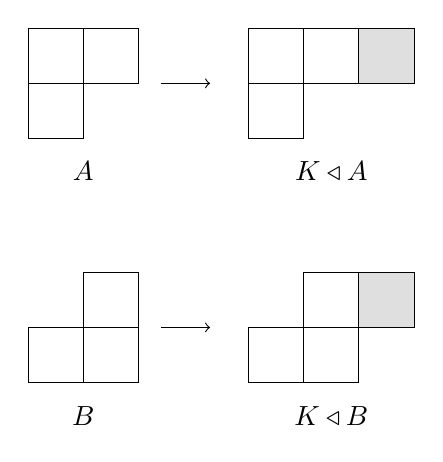
\begin{tikzpicture}[x=0.7cm,y=0.7cm]
 \begin{scope}
  \draw (0,0) rectangle (1,1);
  \draw (1,0) rectangle (2,1);
  \draw (0,-1) rectangle (1,0);
  \node at (1,-1.6) {\(A\)};
  \draw[->] (2.4,0) -- (3.3,0);
  \draw (4,0) rectangle (5,1);
  \draw (5,0) rectangle (6,1);
  \draw (4,-1) rectangle (5,0);
  \filldraw[fill=gray!25] (6,0) rectangle (7,1);
  \node at (5.5,-1.6) {\(K\triangleleft A\)};
 \end{scope}
 \begin{scope}[yshift=-3.1cm]
  \draw (1,0) rectangle (2,1);
  \draw (0,-1) rectangle (1,0);
  \draw (1,-1) rectangle (2,0);
  \node at (1,-1.6) {\(B\)};
  \draw[->] (2.4,0) -- (3.3,0);
  \draw (5,0) rectangle (6,1);
  \draw (4,-1) rectangle (5,0);
  \draw (5,-1) rectangle (6,0);
  \filldraw[fill=gray!25] (6,0) rectangle (7,1);
  \node at (5.5,-1.6) {\(K\triangleleft B\)};
 \end{scope}
\end{tikzpicture}
\caption{The same cell cap in \Cref{ex:same-cell-cap}.  Shaded cells are
added by the literal \(00\)-splice.  The top beta changes from three to
four; no new row is introduced.  The common row-column beta remains at
one in the upper pair and at two in the lower pair.}
\label{fig:cell-splice}
\end{figure}

\begin{theorem}[Fixed-cap rigidity]\label{sc:fixed-cap}
Let \(B,B'\) be connected normalized skew diagrams and \(K\) the same
fixed literal connected cap.  If
\[
 s_B=s_{B'},\qquad s_{K\triangleleft B}=s_{K\triangleleft B'},
\]
then \(B=B'\) literally.
\end{theorem}
\begin{proof}
We use strong induction on the child span \(c\), uniformly over every
actual connected cap.  The common whole function supplies the common
span, row count, and signed corner by \Cref{sc:row-degree}.  Put
\(Q=G_B-G_{B'}\).  The two whole identities become
\begin{equation}\label{sc:fcp-observations}
 [z^c]\mathsf H Q=0,
 \qquad [z^{c+a}]\mathsf H C_KQ=0.
\end{equation}
Every coefficient of \(Q\) uses raw letters of index below \(c\).
If its current raw ceiling is \(R\), put \(R'=\max(R,a-1)\).
Taking the independent coefficients of
\(h_{R'+1},\ldots,h_{c+a}\) in the second equation, and removing
\(C_K\) successively from its constant term one, gives
\begin{equation}\label{sc:fcp-prefix-zero}
 Q_j=0\qquad(j<c+a-R').
\end{equation}
If \(R<a\), this already gives \(Q=0\).

We next identify the proper-corner components in decreasing order of
their actual positions.  Suppose all higher components have already
been identified literally.  Let \(P\) be their entire common proper
matrix, including its cross entries, with largest row \(m_0\), least
column \(b\), and span \(S=m_0-b\).  For an empty prefix omit the
corresponding rows and equations.  Let \(t\) be the largest remaining
proper row on either side.  The lower equations are triangular with
respect to the prefix, so their full coefficient difference uses raw
letters only through \(t\).  Subtraction of the complete prefix equations
gives
\begin{equation}\label{sc:fcp-prefix-solve}
 Q_{\mathrm{prefix}}
   =-P^{-1}\left(\sum_{j<b}h_{x-j}Q_j\right)_{x\in\operatorname{rows}P}.
\end{equation}
If \(L>\max(S,t)\), neither \(P\) nor the lower coefficients depends on
\(h_L\).  Differentiating a cross entry can only expose \(Q_{x-L}\),
which is zero by \eqref{sc:fcp-prefix-zero}, because
\(x-L\le m_0-L<c+a-L\).  Descending the raw ceiling in the entire
equation therefore earns \(R=\max(S,t)\).  If \(S\ge t\), the zero
range reaches beyond \(b\), killing the lower part and then the prefix.
Otherwise \(R=t\ge a\).

At \(h_t\), all remaining proper matrix entries have index strictly
below \(t\).  The differentiated crossing entries in
\eqref{sc:fcp-prefix-solve} again multiply coefficients already in
the zero range.  The derivative of the first equation in
\eqref{sc:fcp-observations} has no direct term, since \(Q_{c-t}=0\).
It consequently compares the two complete inverse columns selected
by the next actual row \(t\).  If this row were absent on one side,
the other would be a nonzero feasible Jacobi--Trudi coface, which is
impossible.

Let \(E,E'\) be the next strict proper blocks at \(t\).  A block with
function one is its actual unit.  In the full triangular inverse
column every lower suffix determinant cancels as a whole.  The
remaining connected numerator has flags
\begin{equation}\label{sc:fcp-numerator-flags}
 X_N=\{c\}\cup\operatorname{rows}P
             \cup(\operatorname{rows}E\setminus\{t\}),
 \qquad Y_N=\operatorname{cols}P\cup\operatorname{cols}E.
\end{equation}
Its positivity and connectedness follow by retaining the original
prefix interval and the strict component interval.  Its span is
larger than that of every denominator component.  Unique
factorization and connected primeness therefore give equal functions
of \(E,E'\) and equal functions of their whole connected numerators.
For a unit this identifies the unit literally.  Otherwise equal
span gives their common least column \(b_0\).

The lists
\begin{equation}\label{sc:fcp-recursive-cap}
 X_{K_E}=\{c-t\}\cup(\operatorname{rows}P-t),
 \qquad Y_{K_E}=(\operatorname{cols}P-t)\cup\{0\}
\end{equation}
form an actual connected cap.  After translation by \(b_0\), the
numerators in \eqref{sc:fcp-numerator-flags} are literally
\(K_E\triangleleft E\) and \(K_E\triangleleft E'\).
The child span is \(t-b_0<c\).  The induction hypothesis identifies
the two blocks literally, and the common prefix can be extended.
Every extension removes a proper block; the process terminates.
Thus \(Q=0\).  Its support identifies all columns, and the numerator
test in \eqref{sc:atlas-support} identifies all proper rows.  The
common top completes the literal equality of \(B\) and \(B'\).
\end{proof}

\section{Complete unit restoration}\label{sec:unit-restoration}

\subsection{The complete unit expansion and finite injectivity}

Deleting a common full row and column beta preserves the boundary
height word.  Deleting all common betas therefore gives a connected
zero-free diagram of the same span and area, called the zero-free
core.  The deleted positions are actual vacancies of that core.

\begin{lemma}\label{sc:unit-expansion}
Scale every positive raw letter by \(\epsilon\) while keeping every
genuine unit coherent.  If \(A\) has row rank \(r\) and \(u\) common
row-column positions, then
\begin{equation}\label{sc:core-leading-term}
 s_A=\sigma_A\epsilon^{r-u}
            (s_{A_0}+O(\epsilon))
\end{equation}
at \(\vartheta=1\), where \(A_0\) is its actual zero-free core and \(\sigma_A\)
is the actual simultaneous sorting sign.  Its complete coframe is
regular at \(\epsilon=0\), with leading term the core coframe.
For coequal \(A,B\), the core functions and sorting signs agree and
their unit counts agree.

At a zero-free core with coframe \(g\) and proper matrix
\(T=(U_{i-s})_{i\in I,s\in S}\), write
\(P^+=[Ug]_{<M}\), with \(U_0=0\).  A restoration at a genuine vacancy
\(b\) has complete first coframe increment
\begin{equation}\label{sc:vacancy-pulse}
 \delta^{(b)}=-P^+_b\left(
 z^b-\sum_{s\in S}(T^{-1}v_b)_s z^s\right),
 \qquad v_b=(U_{i-b})_{i\in I}.
\end{equation}
For any rational weights \(\rho_b\) in the full raw field,
\(\delta=\sum_b\rho_b\delta^{(b)}\) satisfies
\[
 \delta_0=0,\qquad [U\delta]_i=0\ (i\in I),\qquad
 \delta_b=-\rho_bP^+_b
 \quad\text{at each genuine vacancy }b.
\]
In particular, a nonzero mask gives a nonzero complete tangent.
\end{lemma}
\begin{proof}
Collect the true unit rows and columns simultaneously.  Their full
block has diagonal one and off-diagonal entries of positive
\(\epsilon\) order.  Its Schur complement has leading term the
complete core matrix, with the corresponding power of \(\epsilon\).
This proves \eqref{sc:core-leading-term} and the regularity of the
coframe after the core proper-corner powers are factored.  It keeps
the entire inverse of the unit block.

Equal whole functions have equal row counts by
\Cref{sc:row-degree}.  Their least nonzero \(\epsilon\) powers give
equal unit counts and proportional core functions with their actual
signs.  Evaluation of actual skew Schur functions on a sufficiently
large positive alphabet fixes the signs and gives whole core
equality.

For one restored vacancy, the first new native equation is
\(\delta_b=-[Ug]_b=-P^+_b\).  The old proper rows acquire the
contribution \(v_b\delta_b\).  Solving the entire old system therefore
gives the correction \(P^+_bT^{-1}v_b\), which proves
\eqref{sc:vacancy-pulse}.  Linearity proves the displayed native
equations for any weights.  No other vacancy contributes at the
new column \(b\), and \(P^+_b\ne0\) by the actual numerator atlas.
\end{proof}

\begin{lemma}\label{sc:finite-injectivity}
Let \(g\) be the complete coframe of an actual connected normalized
diagram of span \(M\).  Let \(\delta\) be any polynomial over its full
raw field with \(\deg\delta<M\), \(\delta_0=0\), and
\([H\delta]_i=0\) at every original proper row.  For
\(0\le a\le M-1\),
\[
 \mathcal T_{g,\delta}(z^aH)=0\quad\Longleftrightarrow\quad\delta=0.
\]
If the diagram is zero-free, the same assertion with \(H\) replaced
by \(U\), \(U_0=0\), holds for \(0\le a\le M-2\), provided its native
equations are \([U\delta]_i=0\).  No support restriction on
\(\delta\) is required.  Vanishing modulo \(z^{2M-1}\) suffices in
both statements.
\end{lemma}
\begin{proof}
For the first statement, set \(P=[Hg]_{<M}\).  The polynomial
\(z^aP_{<M-a}\) is coprime to \(g\): \(g(0)=1\) removes \(z^a\), and
specializing the independent positive numerator coordinates to zero
leaves \(\vartheta\ne0\).

In the zero-free case, put \(P^+=[Ug]_{<M}\).  The change from the
coherent numerator coordinates to \(P^+\) subtracts the corresponding
coframe coordinates and is invertible with \(g\) fixed.  The available
coefficients of \(P^+\) remain independent.  Its coefficient at one
is available: an actual proper row at one would require column one
and would be a unit.  This independent coordinate survives in
\(z^aP^+_{<M-a}\) for \(a\le M-2\).  Modulo any irreducible factor of
\(g\), its coefficient is \(z^{a+1}\ne0\).  Thus this product too is
coprime to \(g\); \(g=1\) causes no exception.

Write \(W=H\) or \(U\).  A zero wedge gives
\[
 \delta=gR,\qquad
 [z^aW\delta]_{<M}=R[z^aWg]_{<M},\qquad R_0=0.
\]
If \(R\ne0\), let \(e=\deg R\ge1\) and let \(j\) be the largest
available numerator position below \(M-a\).  It exists: \(j\ge0\)
in the first case and \(j\ge1\) in the second.  The right side has
exact degree \(a+j+e\).  If this is at least \(M\), clipping is
contradicted.  Otherwise \(j+e\) is below \(M-a\) and is greater than
every available numerator position, hence is an original proper row.
The left coefficient there is the required zero \([W\delta]_{j+e}\),
whereas the right leading coefficient is nonzero.  Thus \(R=0\).
Both sides are whole polynomials of degree at most \(2M-2\), giving
the asserted finite precision.
\end{proof}

\subsection{A genuine linearized fixed-cap theorem}

The next theorem supplies the first nonzero whole-unit grade in the
cell-splice comparison.  Unlike \Cref{sc:finite-injectivity}, it concerns
two actual polynomial observations, and its weights are constants.

Let \(B\) be a zero-free connected diagram with complete matrix \(M_B\).
At a genuine vacancy \(b\), let
\(a_b=(h_{x-b})_{x\in X_B}\) and
\(b_b=(h_{b-y})_{y\in Y_B}\), and put
\begin{equation}\label{sc:restoration-polynomial}
 \dot s_B^{(b)}=-b_b\,\operatorname{adj}(M_B)\,a_b.
\end{equation}
If \(\sigma_b\) is the actual sorted insertion sign, the complete
bordered determinant is
\[
 s_{B+b}=\sigma_b\bigl(s_B+\dot s_B^{(b)}\bigr)
\]
at physical unit one.  More precisely, scaling positive letters by
\(\epsilon\) and the new unit by \(\nu\) gives
\begin{equation}\label{sc:bordered-grade}
 s_{B+b}=\sigma_b\left(
 \nu\epsilon^r s_B+\epsilon^{r+1}\dot s_B^{(b)}\right),
 \qquad r=\operatorname{rank}M_B.
\end{equation}
Thus \(\dot s_B^{(b)}\) has the same weighted degree as \(s_B\) and
ordinary positive-letter degree \(r+1\).

For constants \(\rho_b\in\Q\) supported on the genuine vacancies,
write \(\dot s_B=\sum_b\rho_b\dot s_B^{(b)}\).  On a fixed cap
splice use the same weights at the same low positions.  The extra
row and column insertion count is even, so the normalized signs
agree.

\begin{theorem}[Zero-free linearized fixed-cap rigidity]
\label{sc:linearized-cap}
Let \(B\) and \(K\) be actual connected zero-free diagrams, and use the
same constant vacancy weights on \(B\) and on the actual splice
\(K\triangleleft B\).  If
\[
 \dot s_B=0,\qquad \dot s_{K\triangleleft B}=0
\]
as whole polynomial identities, then every \(\rho_b\) is zero.
\end{theorem}
\begin{proof}
Write \(m\) for the span of \(B\) and \(v\) for that of \(K\).
Let \(D_0\) be the complete proper matrix of \(B\), \(\kappa\) its signed
determinant, and \(G\) its complete coframe.  The exact first variation
\(Q\) of the coframe includes both the original native columns and
the new vacancy columns.  The bordered solve gives
\begin{equation}\label{sc:linearized-coframe}
 Q=-\sum_b\rho_bP_b
 \left(z^b-\sum_{s\in S_B}(D_0^{-1}v_b)_sz^s\right),
 \quad P_b=[\mathsf HG]_b,\quad v_b=(h_{i-b})_{i\in I_B}.
\end{equation}
In particular \(Q_0=0\), \(\deg Q<m\), \(Q_b=-\rho_bP_b\) at a
vacancy, and \([\mathsf HQ]_i=0\) at every original proper row.

All coefficients of \(Q\) and \(\kappa\) have raw ceiling below \(m\).
The unique top-letter coefficient of \(\dot s_B=0\) gives
\(\dot\kappa=0\), and its remaining whole equation gives
\([\mathsf HQ]_m=0\).  Differentiating the exact fixed-cap identity
\eqref{sc:splice-identity} then gives
\begin{equation}\label{sc:linearized-observations}
 [\mathsf HQ]_m=0,
 \qquad [\mathsf HC_KQ]_{m+v}=0.
\end{equation}
If \(Q\) has raw ceiling \(R\), successive comparison of the genuine
high-letter coefficients in the second equation gives
\begin{equation}\label{sc:linearized-zero-range}
 Q_j=0\qquad(j<m+v-\max(R,v-1)).
\end{equation}
This is the same triangular removal of the constant-one coframe
\(C_K\) as before.  If \(R<v\), all coefficients vanish.

We use strong induction on \(m\), uniformly over actual zero-free
caps.  Suppose the restoration weights in all higher strict blocks
have already been removed, and let \(P\) be their entire fixed proper
prefix, including its crossing blocks.  Write \(m_0\) for its largest
row, \(a\) for its least column, and \(S=m_0-a\); omit an empty prefix.
Let \(t\) be the largest remaining proper row and \(b_{\max}\) the
largest remaining vacancy, using zero for an empty set.  The lower
coframe coefficients have raw ceiling at most \(\max(t,b_{\max})\).
Their full prefix compensation is
\begin{equation}\label{sc:linearized-prefix}
 Q_{\mathrm{prefix}}
   =-P^{-1}\left(\sum_{j<a}h_{x-j}Q_j\right)_{
                           x\in\operatorname{rows}P}.
\end{equation}
If a raw ceiling \(L\) exceeds \(\max(S,t,b_{\max})\), every
differentiated crossing entry multiplies \(Q_{x-L}\), which is zero
by \eqref{sc:linearized-zero-range}.  The whole prefix equation
therefore has zero derivative in \(h_L\).  Descending earns
\(R=\max(S,t,b_{\max})\).  If \(S\ge\max(t,b_{\max})\), the zero
range passes \(a\), so the tail and then the prefix vanish.  Otherwise
\(R=\max(t,b_{\max})>S\); when \(R\ge v\) the zero range includes
\begin{equation}\label{sc:linearized-direct-zeros}
 Q_{m-R}=0,\qquad Q_{x-R}=0
       \quad(x\in\operatorname{rows}P).
\end{equation}

There are two next-head cases.  First suppose \(R=b_{\max}>t\) and
write \(b=R\).  Every remaining baseline proper row is below \(b\);
its entry in the restored column is genuinely zero.  Every weighted
vacancy lies below the least prefix column, so \(b<a\), and
\(P_b-h_b\) is a function of lower raw letters.  Differentiating
\eqref{sc:linearized-coframe} and
\eqref{sc:linearized-prefix} in \(h_b\), all crossing derivatives
multiply the zeros in \eqref{sc:linearized-direct-zeros}.
The surviving pulse is \(-\rho_b\) at the new column and its full
prefix correction.  Differentiating the whole top equation gives
\begin{equation}\label{sc:gap-coface}
 \rho_b\left(h_{m-b}
  -H_{m,\operatorname{cols}P}P^{-1}H_{\operatorname{rows}P,b}
       \right)=0.
\end{equation}
The numerator in parentheses has actual rows
\(\{m\}\cup\operatorname{rows}P\) and columns
\(\operatorname{cols}P\cup\{b\}\).  On \([b,m)\) its height is one
plus the prefix height, with the two genuine singleton ends.  It is
therefore an actual connected skew diagram with nonzero Schur
function.  Its full denominator is \(\det P\).  Consequently
\(\rho_b=0\).  This also handles the case with no proper block left.

Now suppose \(R=t>b_{\max}\).  Let \(E\) be the next actual zero-free
strict block, with head \(t\) and least column \(a_0>0\), closed by a
cut immediately after it, so that no further proper index overlaps
\(E\) from above.  The complete
proper matrix has triangular form
\[
 \begin{pmatrix}
 P&B_{PE}&B_{PL}\\
 0&E&B_{EL}\\
 0&0&L
 \end{pmatrix}.
\]
The inverse column selected by row \(t\) has no component in the
lower suffix \(L\).  After all suffix factors cancel as a whole, its
top row-replacement quotient is, with its actual sign,
\(s_N/(\det P\,s_E)\), where
\[
 X_N=\{m\}\cup\operatorname{rows}P
                 \cup(\operatorname{rows}E\setminus\{t\}),
 \qquad Y_N=\operatorname{cols}P\cup\operatorname{cols}E.
\]
Differentiate the whole equation \([\mathsf HQ]_m=0\) in \(h_t\).
The direct term and the differentiated crossings vanish by
\eqref{sc:linearized-direct-zeros}.  A restoration in \(L\) cancels
in the complete triangular quotient.  A restoration in \(E\) affects
both its determinant and the whole numerator \(N\), with the same
weight.  Multiplication by all actual denominators gives precisely
\begin{equation}\label{sc:strict-block-variation}
 s_E\dot s_N-s_N\dot s_E=0.
\end{equation}
The numerator is connected: the original prefix interval joins the
true strict block with its singleton end caps.  The lists
\[
 X_{K_E}=\{m-t\}\cup(\operatorname{rows}P-t),
 \qquad Y_{K_E}=(\operatorname{cols}P-t)\cup\{0\}
\]
define an actual connected zero-free cap.  After translating by
\(a_0\), one has literally \(N=K_E\triangleleft E\).  Its span
\(m-a_0\) exceeds the child span \(t-a_0\).

Thus \(s_E,s_N\) are coprime connected functions, and
\eqref{sc:strict-block-variation} implies \(s_E\mid\dot s_E\).
Since \(E\) is zero-free, \eqref{sc:bordered-grade} makes
\(\dot s_E\) have the same positive weighted degree as \(s_E\) and
ordinary positive-letter degree one greater.  A polynomial quotient
would have weight zero and ordinary degree one, which is impossible
in positive-weight letters.  Hence \(\dot s_E=0\), and then
\(\dot s_N=0\).  The induction hypothesis applies to the smaller
child \(E\) and the actual zero-free cap \(K_E\).  It removes all
restoration weights in \(E\).  The sorted insertion parity changes
by an even number, so these are the original weights.

Extend the fixed prefix and repeat.  Each remaining vacancy is in
a genuine gap or a genuine strict block, so the process terminates.
Equivalently, at its conclusion \(Q=0\), and
\(Q_b=-\rho_bP_b\) at each previously absent native column forces
every \(\rho_b=0\), because the actual feasible numerator \(P_b\) is
nonzero.
\end{proof}

\subsection{The first cell-splice grade and finite shifts}

\begin{lemma}
\label{sc:splice-nonzero}
Let \(V\) be an actual connected diagram that is not its normalized
rotation.  At physical normalization put
\[
 J_2=s_{V\triangleleft\mathrm{CELL}}
              -s_{\mathrm{CELL}\triangleleft V}.
\]
Let its zero-free core have \(k\) rows and let \(u\) be the number of actual
units.  Scale the positive alphabet by \(\varepsilon\), retaining the
coherent unit \(\nu\ne0\).  Then \(J_2\) is nonzero.  Its first nonzero
grade is
\[
 \lambda=k\quad\text{if the core is not self-rotating},\qquad
 \lambda=k+1\quad\text{if the core is self-rotating}.
\]
The full absolute adjugate difference between \(V\) and its rotation has
no grade below \(\mu=\lambda-1\).  Consequently every supplied current
formed by a single positive raw contraction of that whole array has
order at least \(\lambda\).
\end{lemma}
\begin{proof}
The full simultaneous unit Schur complement gives, with the actual
sorting sign \(\tau\),
\begin{equation}\label{sc:whole-unit-series}
 s_V=\tau\nu^u\varepsilon^k
 \left(s_B+\frac\varepsilon\nu
            \sum_{b\in U_V}\dot s_B^{(b)}+O(\varepsilon^2)\right).
\end{equation}
It applies to both literal cell splices with all unit positions retained.
If \(B\) is not self-rotating, rotating one of the splice observations
turns vanishing of its leading \(J_2\) into equality of the same
literal-cell extensions of \(B\) and \(B^*\).  They already have equal
whole functions.  \Cref{sc:fixed-cap} would give \(B=B^*\), a
contradiction.  Thus grade \(k\) is nonzero.

If \(B=B^*\), the constant core observations coincide.  Since \(V\ne V^*\),
the actual weights
\(\rho_b=\mathbf1_{U_V}(b)-\mathbf1_{U_V}(M-b)\) are not all zero.
The whole equality \(s_V=s_{V^*}\) at the next grade gives
\(\dot s_B=0\).  If the grade-\(k+1\) cell-splice difference vanished,
the same weights and sorting signs would give
\(\dot s_{\mathrm{CELL}\triangleleft B}=0\).
Both the child and this cap are zero-free, so
\cref{sc:linearized-cap} would make every \(\rho_b=0\).
Thus this next grade is nonzero.

For completeness, place the common unit flags last in both orders in
the whole adjugate.  Its first possible grade is \(k-1\); at that grade
only core-to-core coefficients remain, and the entire absolute array
is \(\tau\nu^u\operatorname{adj}(\operatorname{JT}(B))\).
For a self core the corresponding entire arrays agree, including the
sorting sign obtained from the equal whole determinants.  The next
grade is attained at any actual unit position present on one side and
absent on its rotation: delete that row and column zero and match all
remaining actual units.  The remaining weak flags have nonnegative
heights and disjoint lists, hence a nonzero positive-letter determinant
of degree \(k\).  The other array has no entry at that actual row.
If the core is not self, the analogous unmatched core boundary cofactor
is already nonzero at grade \(k-1\).
This proves the asserted whole-array orders.  Multiplication by one
positive raw letter raises the order by one; the complete contraction
cannot create a lower grade.  This last conclusion refers to the
supplied contraction of the whole array, not to independent observations
of its tied entries.
\end{proof}


\section{Finite stationary separation}\label{sec:stationary}

The exponent in this section is an integer at least two, not a
composition period.  The coframes belong to actual connected diagrams
with equal whole Schur functions, at their supplied common span.

\subsection{Highest-component matching}

The highest strict proper component has a head \(m\), least column \(a\),
and span \(L=m-a\).  The inverse column selected by its head has the form
\begin{equation}\label{sc:component-column}
 -z^ag/k,
 \qquad k=[Hg]_L,
\end{equation}
where \(g\) is the component's own right coframe.  This is Cramer's
rule applied to the complete block-triangular proper matrix: the
selected inverse column has zero lower-suffix entries, and all lower
suffix factors cancel as a whole.  For a true unit, \(L=0\), \(g=1\), \(k=\vartheta\).

\begin{lemma}\label{sc:component-remainder}
For an actual connected component of span \(L\ge2\) and any integer
\(p\ge2\),
\begin{equation}\label{sc:nonzero-remainder}
 [H^pg]_L=p\vartheta^{p-1}k+\alpha,
 \qquad k=H_L+k_0,
\end{equation}
where \(k_0\) and \(\alpha\) are independent of \(H_L\), and \(\alpha\ne0\).
\end{lemma}
\begin{proof}
The independence of \(H_L\) is immediate from the complete proper
solve.  On the child's neutral top \(k=0\), the remainder becomes
\([P^p/g^{p-1}]_L\), where \(P=[Hg]_{<L}\) and \(P_0=\vartheta\).
Use the actual independent coordinates of \Cref{sc:atlas}.
If \(g\ne1\), let \(b\) be its least native column and write
\(L=nb+j\), \(0\le j<b\).  Actual feasibility makes
\(P_1,\ldots,P_{b-1}\) available.  For \(j=0\), the coefficient of
the independent monomial \(g_b^n\) is
\((-1)^n\binom{p+n-2}{n}\vartheta^p\); for \(j>0\), that of
\(P_jg_b^n\) is
\((-1)^np\binom{p+n-2}{n}\vartheta^{p-1}\).  Both are nonzero.
If \(g=1\), the component is a row.  At \(L=2\), the coefficient of
\(P_1^2\) is \(\binom p2\vartheta^{p-2}\), and at \(L\ge3\), that of
\(P_1P_{L-1}\) is \(p(p-1)\vartheta^{p-2}\).  This proves nonvanishing,
including the two-cell row at \(p=2\).
\end{proof}

\begin{lemma}
\label{sc:top-matching}
Let \(A,B\) be actual connected coequal diagrams of span \(M\), both
having proper row \(m=M-1\).  Put \(\Delta=C-G\).  Suppose, for an
integer \(p\ge2\),
\[
 [H^p\Delta]_m=0,
 \qquad
 \partial_{H_m}\bigl([H^p\Delta]_M
                      -\Delta_1[H^pG]_m\bigr)=0.
\]
Then their highest strict proper components agree literally in
position.  Moreover \(\partial_{H_m}\Delta=0\) and \(\Delta_1=0\).
\end{lemma}
\begin{proof}
Put \(y=H_m\).  Let the two top components have least columns \(a,b\),
spans \(L=m-a\), \(L'=m-b\), coframes \(g,c\) and quotients \(k_E,k_F\).
By \eqref{sc:component-column},
\[
 \partial_yG=-z^ag/k_E,\qquad
 \partial_yC=-z^bc/k_F.
\]
The coefficient of \(y\) in the first observation gives
\begin{equation}\label{sc:component-ratio}
 \frac{[H^pg]_L}{k_E}=\frac{[H^pc]_{L'}}{k_F}.
\end{equation}
The explicit derivative of \(H^p\) multiplies \(\Delta_0=0\).
For \(L\ge2\), \Cref{sc:component-remainder} gives a genuine pole
in the independent top letter \(H_L\).  If \(L>L'\), the right side is
independent of that letter, an impossibility.  The remaining unequal
case, \(L=1,L'=0\), compares \(p\vartheta^{p-1}\) with \(\vartheta^{p-1}\) and is also
impossible.  Interchanging the diagrams gives \(L=L'\) and \(a=b\).

For \(L=0\), both components are the same true unit:
\(g=c=1\), \(k_E=k_F=\vartheta\).
For \(L=1\), both are the same cell:
\(g=c=1\), \(k_E=k_F=H_1\).
In either case \(a=b\), and the complete selected inverse columns,
including their zero lower suffixes, agree.  Hence
\(\partial_y\Delta=0\).  Differentiating the whole coequal identity
gives
\[
 0=\partial_y[H\Delta]_M
   =[z^{M-1}\Delta]_M+[H\partial_y\Delta]_M=\Delta_1.
\]
This closes both small cases with their actual unit or cell denominator.

For \(L\ge2\), write \(k_E=H_L+k_{E,0}\) and
\(k_F=H_L+k_{F,0}\).  Cross-multiplication in
\eqref{sc:component-ratio} first gives equal nonzero remainders
and then \(k_{E,0}=k_{F,0}\).  Thus \(k_E=k_F=:k\).
Connected primeness and coprimality with the full proper corners
identify the actual child functions and their signed corners; primitive
normalization fixes the scalar.

Assume \(L\ge2\), and put \(\delta=c-g\),
\(A_p=[H^pg]_L\), \(B_p=[H^p\delta]_{L+1}\),
\(V=[H\delta]_{L+1}\).  These expressions are independent of \(y\).
Also \(\Delta_1\) is \(y\)-independent, since \(\delta_0=0\) and \(a\ge1\).
The second supplied observation gives
\(B_p=\Delta_1A_p\).  Differentiating the whole equality
\([H\Delta]_M=0\) gives \(V=\Delta_1k\).  In particular,
\begin{equation}\label{sc:component-next-relation}
 kB_p=VA_p.
\end{equation}
Set \(x=H_L\) and write
\[
 k=x+k_0,\quad V=x\delta_1+v_0,\quad
 A_p=p\vartheta^{p-1}k+\alpha,\quad
 B_p=p\vartheta^{p-1}V+\beta.
\]
All subscript-zero terms and \(\alpha,\beta\) are independent of \(x\),
and \(\alpha\ne0\).  Equation \eqref{sc:component-next-relation}
becomes \(\beta k=\alpha V\).  Comparing \(x\) and then its constant
coefficient gives \(V=\delta_1k\).

Let \(\kappa_*\) be the common signed child corner.  The difference
of the two actual same-cell splice functions is the polynomial
\[
 B_{\mathrm{cell}}
 =\kappa_*([Hg]_{L+1}-[Hc]_{L+1})=-s_E\delta_1.
\]
The product \(\kappa_*\delta_1\) is polynomial.  Since
\(\gcd(s_E,\kappa_*)=1\), the connected function \(s_E\) divides
\(B_{\mathrm{cell}}\).  Both splices add one cell without increasing
the child row count, so \(B_{\mathrm{cell}}\) has positive row degree
at most that of \(s_E\).  A nonzero quotient would have positive
weighted degree one and therefore positive ordinary degree,
contradicting \Cref{sc:row-degree}.  Hence \(B_{\mathrm{cell}}=0\).
The actual children have equal whole functions and equal same-cell
splice functions.  \Cref{sc:fixed-cap} identifies them literally.
Thus \(g=c\), \(\partial_y\Delta=0\), and \(\Delta_1=0\) follows from
\(V=\Delta_1k\).
\end{proof}

\begin{lemma}\label{sc:top-support}
Suppose two actual coequal diagrams have their highest strict proper
components literally matched in position, with least column \(a\).
If their complete coframes differ, then
\(1\le\ord_z(C-G)\le a-2\).
\end{lemma}
\begin{proof}
Let \(P\) be the complete common top matrix and
\(\delta=[C-G]_{<a}\).  Subtraction of its full native equations gives
\[
 ((C-G)_s)_{s\in\operatorname{cols}P}
   =-P^{-1}\left(\sum_{j<a}H_{x-j}\delta_j\right)_{
                         x\in\operatorname{rows}P}.
\]
Thus a nonzero difference starts below \(a\).  If it started at
\(a-1\), the exact native support would identify all columns below
\(a-1\), and the numerator-zero test would identify all rows there.
The common top identifies both flags at or above \(a\).  Equal total
row counts then determine row membership at \(a-1\), and equality of
the proper row and column counts determines column membership there.
All flags would agree, contradicting the distinct coframes.
\end{proof}

\subsection{A finite pole calculation}

The potential in the following theorem is an arbitrary fixed rational
function.  Its value is not calibrated in advance.  The proof uses only
coefficients already present at the stated finite horizon.

\begin{theorem}[One-power stationary separation]\label{sc:positive-power}
In the domain of \Cref{sc:coequal-data}, let \(p\ge2\) be an integer and
\(r(x)\in K(x)\).  If
\begin{equation}\label{sc:power-equation}
 R(z):=\mathcal T_{G,C}(zH^p)+zD r(H)=0\pmod {z^{2M}},
\end{equation}
then \(A=B\) literally.  Conversely, literal equality makes the identity
hold for every such rational potential.
\end{theorem}
\begin{proof}
Suppose \(A\ne B\), and put \(m=M-1\) and \(\Delta=C-G\).
Because \(zD r(H)\) has order at least \(M+2\), the first two retained
coefficients give
\begin{equation}\label{sc:two-endpoints}
 E_0=[H^p\Delta]_m=0,\qquad
 E_1=[H^p\Delta]_M-\Delta_1[H^pG]_m=0.
\end{equation}
Indeed, direct subtraction of the two discarded tails gives
\[
 [\mathcal T(zH^p)]_M=-E_0,\qquad
 [\mathcal T(zH^p)]_{M+1}=-E_1-G_1E_0.
\]
The corresponding coefficient is retained also when \(M=3\).

We first earn the maximal-row incidence.  If exactly one proper row
set contains \(m\), the full derivative of \(E_0\) in \(y=H_m\) is, up to
sign,
\[
 \frac{[H^pg]_L}{k},
\]
where \(g\) and \(k=[Hg]_L\) belong to its actual highest strict proper
component.  This is nonzero: for a positive component its numerator
has coefficient \(p\vartheta^{p-1}\) at \(H_L\), and a true unit gives
\(\vartheta^{p-1}\).  The inverse-column calculation is
\eqref{sc:component-column}.  If neither proper row set contains \(m\),
the complete coframes are independent of \(y\), and differentiation of
\eqref{sc:power-equation} yields
\[
 R_y=-z^M\Delta r(H)\pmod {z^{2M}}.
\]
The derivative of the potential itself starts beyond the retained
window.  If \(r\ne0\), then \(r(\vartheta)\ne0\) because \(\vartheta\) is transcendental,
and the first term of this product is visible.  Thus \(r=0\).
Now \(\mathcal T(zH^p)=0\) is a whole polynomial identity.  Coprimality
of \(G,C\) implies \([zH^pG]_{<M}=AG\) with \(\deg A\le M-2\).
Division by \(G\), whose constant is one, gives
\(A=zH^p\pmod {z^M}\).  Its degree-\(M-1\) coefficient contains the
nonzero independent-letter term \(p\vartheta^{p-1}H_{M-2}\), a contradiction.
Consequently both proper row sets contain \(m\).

By \Cref{sc:top-matching}, \eqref{sc:two-endpoints} identifies their
highest strict proper components literally in position.  Write \(a\) for
the common least column, \(L=m-a\) for its span, \(g\) for its coframe,
and \(k=[Hg]_L\) for its quotient.  A true unit has \(L=0\), \(g=1\),
\(k=\vartheta\).  The complete inverse columns agree:
\begin{equation}\label{sc:common-top-column}
 G=G_0+yv,\quad C=C_0+yv,\quad
 v=-\frac{z^ag}{k},\quad \partial_y\Delta=0.
\end{equation}
The support bound in \Cref{sc:top-support} gives
\begin{equation}\label{sc:needed-support}
 d:=\ord_z\Delta\le a-2.
\end{equation}
Put \(h=H-yz^m\).  Differentiating the whole operator, including its
discarded tails, gives
\[
 D_y=-\mathcal T_{\Delta,v}(h)-z^m\Delta.
\]
The second term is the parent correction.  Since the whole \(D_y\) has
order at least \(M+1\), both the explicit \(r'(H)\) term and the replacement
of \(r(H)\) by \(r(h)\) lose only degrees at least \(2M+1\).  Substituting
\eqref{sc:common-top-column}, and using \(M-a=L+1\), therefore gives
\begin{align}
 R_y=\frac{z^{a+1}}{k}\bigl\{&
   \Delta[h^pg]_{<L}-g[h^p\Delta]_{<M-1}\notag\\
 &+r(h)\bigl(\Delta[hg]_{<L}-g[h\Delta]_{<M}\bigr)
 \bigr\}\pmod {z^{2M}}.\label{sc:complete-pole-bracket}
\end{align}
In this expression the term \(kz^L\Delta\) from the first clipping has
canceled the parent correction.  It has not been omitted.

At inner degree \(L+d\), the two products containing \(\Delta\) are
unclipped, since \(L+d\le M-3\).  Thus
\begin{equation}\label{sc:first-pole-jet}
 [z^{M+d}]R_y
   =-\Delta_d\left(\frac{[h^pg]_L}{k}+r(\vartheta)\right).
\end{equation}
This coefficient lies strictly below \(2M\).

\smallskip\noindent\emph{A component of span \(L\ge2\).}
\Cref{sc:component-remainder} writes
\[
 [h^pg]_L=p\vartheta^{p-1}k+\alpha,
 \qquad k=H_L+k_0,\qquad \alpha\ne0,
\]
where \(\alpha,k_0\) are independent of \(H_L\).  Divide
\eqref{sc:first-pole-jet} by the nonzero rational function \(\Delta_d\);
there is no need for \(\Delta_d\) itself to be independent of \(H_L\).
The \(H_L\) coefficient gives \(r(\vartheta)=-p\vartheta^{p-1}\) and the constant
coefficient then gives \(\alpha=0\).  This is impossible.

\smallskip\noindent\emph{The cell, \(L=1\).}
Here \(g=1\), \(k=H_1\),
\(a=M-2\).  Equation \eqref{sc:first-pole-jet} gives
\(r(\vartheta)=-p\vartheta^{p-1}\), hence \(r(x)=-px^{p-1}\) as a rational identity.
With
\[
 Q_1=[h^p\Delta]_{<M-1}-\vartheta^p\Delta
       -ph^{p-1}\bigl([h\Delta]_{<M}-\vartheta\Delta\bigr),
\]
equation \eqref{sc:complete-pole-bracket} becomes
\(R_y=-z^{M-1}Q_1/H_1\).  Below degree \(M-1\), \(Q_1\) is the
product of \(\Delta\) with
\[
 (1-p)h^p+p\vartheta h^{p-1}-\vartheta^p.
\]
The constant and linear terms vanish.  The quadratic coefficient is
\[
 -\binom p2\vartheta^{p-2}H_1^2.
\]
Since \(d\le M-4\), its first surviving product coefficient is retained, and
\begin{equation}\label{sc:cell-second-jet}
 [z^{M+d+1}]R_y=\binom p2\vartheta^{p-2}H_1\Delta_d\ne0.
\end{equation}
This excludes the cell case, including \(p=2\).

\smallskip\noindent\emph{The true unit, \(L=0\).}
Equation \eqref{sc:first-pole-jet}
now gives \(r(x)=-x^{p-1}\).  Both original diagrams have a true unit
at \(m\).  Normalize coherently and set \(H_\epsilon=1+\epsilon U\),
where \(U_0=0\) and its positive coefficients remain independent.
The complete unit Schur complement of \Cref{sc:unit-expansion} gives
\[
 G_\epsilon=g+\epsilon G_1+\cdots,
 \qquad C_\epsilon=c+\epsilon C_1+\cdots,
\]
where \(g,c\) belong to their actual zero-free cores.  Those cores have
equal whole functions and both omit row and column \(m\).  The true
restored \(m\)-columns have first coefficients \(-[Ug]_m\) and
\(-[Uc]_m\).  Hence the coefficient of \(\epsilon\) in \(E_0=0\) is
\begin{equation}\label{sc:unit-first-cap}
 (p-1)([Uc]_m-[Ug]_m)=0.
\end{equation}
Shortening only the cores' top beta from \(M\) to \(m\) leaves their
proper matrices unchanged and produces actual connected zero-free
diagrams.  Their whole functions agree by
\eqref{sc:unit-first-cap}; adjoining the same literal cell on top
recovers the two original cores, whose whole functions also agree.
The nonlinear fixed-cap result in \Cref{sc:fixed-cap} identifies the
cores literally, so \(g=c\).

If the original unit masks agree, the original diagrams are already
equal.  Otherwise their full first difference
\(\delta=C_1-G_1\) is nonzero: at a differing genuine vacancy \(b\) it
has coefficient \(-\rho_b[Ug]_b\), where \(\rho_b\) is the difference
of the two restoration indicators.  All compensating old-column
terms are included in \Cref{sc:unit-expansion}.  In particular,
\(\delta_0=0\) and \([U\delta]_i=0\) at every core proper row.

Write the alternating pair of coframes as
\(G_\epsilon\wedge C_\epsilon=\epsilon W_1+\epsilon^2W_2+\cdots\),
where \(W_1=g\wedge\delta\), and set \(D_1=\mathcal T_{W_1}(U)\).
Here \(\mathcal T\) depends linearly on the alternating pair; this
notation only groups complete coefficients.  Both original maximal
row equations give the entire identity
\begin{equation}\label{sc:native-shift-identity}
 \mathcal T_{G_\epsilon,C_\epsilon}(zH_\epsilon)
       =z\mathcal T_{G_\epsilon,C_\epsilon}(H_\epsilon).
\end{equation}
The \(\epsilon^2\) coefficients of this identity and of
\eqref{sc:power-equation}, respectively, are
\[
 \mathcal T_{W_2}(z)+\mathcal T_{W_1}(zU)-zD_1=0,
 \qquad
 \mathcal T_{W_2}(z)+p\mathcal T_{W_1}(zU)-zD_1=0.
\]
Their difference is \((p-1)\mathcal T_{g,\delta}(zU)=0\).
These are whole polynomials of degree below \(2M\).
Finite zero-free coframe injectivity, \Cref{sc:finite-injectivity},
forces \(\delta=0\), a contradiction.  Every incidence and highest
component case has now been exhausted.
\end{proof}

\subsection{The whole moving potential}

\begin{corollary}\label{cor:stationary-field-descent}
Retain the domain of \Cref{sc:coequal-data}: the actual connected
diagrams \(A,B\) with \(s_A=s_B\), their complete coframes \(G,C\),
the defect \(D=\mathcal T_{G,C}(H)\), and the same supplied \(M\).
Let \(\mathbb F\supseteq K(\vartheta)\) be the neutral coefficient
field, with all retained positive coarse raw letters algebraically
independent over \(\mathbb F\).  Write \(\mathbf H\) for that finite
tuple of letters.  Suppose the supplied whole moving homomorphism is
\[
 \mathcal R:\mathbb F\longrightarrow
       \mathbb F(\mathbf H)[z]/(z^{2M}),\qquad
 \mathcal R|_K=\mathrm{id},\quad
 \mathcal R(\vartheta)=H,\quad
 \mathcal R(a)\equiv a\pmod z\quad(a\in\mathbb F).
\]
It acts on every dependent rational coordinate, including complete
inverse entries; rational substitution is legitimate because every
nonzero denominator has its original nonzero constant term.
If \(c\in K^\times\), \(p\ge2\) is an integer, and
\(\psi_0\in\mathbb F\) satisfies
\begin{equation}\label{sc:whole-field-equation}
 c\mathcal T_{G,C}(zH^p)+zD\mathcal R(\psi_0)=0
                       \pmod {z^{2M}},
\end{equation}
then \(A=B\) literally.
\end{corollary}
\begin{proof}
For a distinct pair put \(\ell=\ord_zD\le2M-2\).  Its retained coefficient
at degree \(\ell+1\) gives
\[
 \frac{\psi_0}{c}
 =-\frac{[z^{\ell+1}]\mathcal T_{G,C}(zH^p)}{D_\ell}.
\]
The left side belongs to \(\mathbb F\), the right side to
\(K(\vartheta,H_1,\ldots,H_{M-1})\).  Raw independence gives
\[
 \mathbb F\cap K(\vartheta,H_1,\ldots,H_{M-1})=K(\vartheta).
\]
Thus \(\psi_0/c=r(\vartheta)\) for a fixed rational function \(r\in K(x)\).
Applying the whole homomorphism, which fixes \(c\), gives
\(\mathcal R(\psi_0)/c=r(H)\).  This contradicts
\Cref{sc:positive-power}.  The argument does not assume that
\(D_{M+1}\) is nonzero.
\end{proof}

The coefficient at \(2M-1\) cannot be discarded: it can be the first
one at which a potential occurs when \(\ord D=2M-2\).
Likewise an amplitude can be divided out only when it belongs to the
fixed, raw-independent field.  A coefficient of the fine field must
move under \(\mathcal R\), just as the returned coordinate does.
An application must establish that its amplitude is in the fixed field
before invoking this corollary.

\begin{example}\label{ex:terminal-coframes}
For \(A=(2,1)\) and \(B=(2,2)/(1)\), the full coherent native
matrices are
\[
 \JT(A)=\begin{pmatrix}H_2&H_3\\ \vartheta&H_1\end{pmatrix},
 \qquad
 \JT(B)=\begin{pmatrix}H_1&H_3\\ \vartheta&H_2\end{pmatrix}.
\]
Both determinants are \(H_1H_2-\vartheta H_3\), and \(M=3\).
Their proper native equations are
\(\vartheta G_1=-H_1\) and \(\vartheta C_2=-H_2\), respectively.
Consequently
\[
 G=1-\frac{H_1}{\vartheta}z,\qquad
 C=1-\frac{H_2}{\vartheta}z^2,\qquad
 D=\frac{H_2(\vartheta H_2-H_1^2)}{\vartheta^2}z^4.
\]
Thus \(\ord D=4=2M-2\), and the first coefficient containing
the moving potential in \(zD\mathcal R(\psi_0)\) has degree
\(5=2M-1\).  This explains the terminal coefficient in this
potential-descent argument; it does not assert that every weaker
recognition test fails.
\end{example}


The specialization \(u=H\) of \eqref{sc:exact-shift-cap} gives
\(\mathcal T(zH)-zD\).  It vanishes exactly when the whole cap
polynomial in that formula vanishes.  The two actual maximal-row equations
in the unit argument supply the separate scalar zeros, which are
sufficient but not necessary for arbitrary coframes.

\section{Unshifted opposite-end exclusion}\label{sec:unshifted}

For a board of span \(M\), use the coherent clock \(\vartheta\ne0\),
independent positive letters \(H_i\), and its two complete coframes
\(G,C\), with constant one.  Put
\[
 P=[HG]_{<M},\quad Q=[HC]_{<M},\quad D=GQ-CP,
 \quad
 \mathcal{T}_{A,B}(F)=A[FB]_{<M}-B[FA]_{<M}.
\]
Every truncation in this section is literal.  In particular
\[
 \mathcal{T}_{G,C}(zH)-zD
   =-z^M\{G[HC]_{M-1}-C[HG]_{M-1}\};
\]
its vanishing is equivalent to the vanishing of the displayed
\emph{whole polynomial}.  Separate scalar-cap zeros are sufficient,
not necessary for arbitrary coframes.

The equation below is unshifted.  It is not
\eqref{sc:power-equation}: moving \(z\) through the finite operator
creates the whole cap term in \eqref{sc:exact-shift-cap}.

\begin{lemma}\label{ph:unshifted-exclusion}
Let \(V\) be an actual connected diagram of span \(M\ge3\), and
let \(G,C\) be its complete right and left coframes, equivalently
the right coframes of \(V,V^*\), in the same coherent raw alphabet.
Retain every proper component and every actual unit.  For an integer
\(p\ge2\), the identity
\[
 \mathcal T_{G,C}(H^p)=p[H^{p-1}D]_{<2M}
\]
at precision \(2M\), including degree \(2M-1\), implies \(V=V^*\).
This assertion concerns opposite ends of one actual board, not
arbitrary coequal coframe pairs.
\end{lemma}
\begin{proof}
Suppose \(V\ne V^*\).
First, a connected \(k\)-row determinant has ordinary positive-letter
degree exactly \(k\).  Its degree-\(k\) component is obtained by replacing
all units by zero.  The substitution \(H_i\mapsto h_{i-1}\), \(i>0\),
turns it into the weak skew determinant obtained by removing one cell
from every row, which is nonzero.  Thus a nonzero polynomial of degree
at most \(k\) and weight greater than the board's area cannot be
divisible by its connected prime.
The actual cell-cap difference \(J_2\ne0\) from
\Cref{sc:splice-nonzero} has these degree and surplus-weight
properties.  Hence it survives the genuine top-neutralization.
After this top-neutralization the complete coframe formula yields
\begin{equation}\label{ph:first-D}
 [z^{M+1}]D=-J_2|_{e=0}/\kappa\ne0
\end{equation}
for an actual nonself board.  This specific conclusion uses the
cell-cap theorem, not merely \(D\ne0\).  We will apply it to actual
connected components in their own fields.

Set \(m=M-1\), \(y=H_m\), and \(H=h+yz^m\), with \(h_m=0\).
Let \(I\) and \(S\) be the proper row and column sets, and let \(\Pi\)
be the complete proper inverse, independent of \(y\).
Define
\[
 a=-\sum_{c\in S}\Pi_{c,m}z^c,\qquad
 b=-\sum_{i\in I}\Pi_{1,i}z^{M-i}.
\]
A missing native port means the zero vector.
Then \(G=G_0+ya\), \(C=C_0+yb\), where the subscript zero means
\(y=0\).  Write \(\Delta=G_0-C_0\),
\(W_0=G_0\wedge C_0\),
\(W_1=a\wedge C_0+G_0\wedge b\), \(W_2=a\wedge b\).
For a wedge \(W=A\wedge B\), put
\[
 \mathcal{E}^{M}_W
   =\mathcal{T}^{M}_{A,B}(h^p)-p h^{p-1}\mathcal{T}^{M}_{A,B}(h),
\]
always at precision \(2M\).
The complete coefficients of the defect are
\begin{align*}
 [y^0]\mathcal{E}&=\mathcal{E}^{M}_{W_0},\\
 [y^1]\mathcal{E}&=\mathcal{E}^{M}_{W_1}
           +p(\vartheta^{p-1}-h^{p-1})z^m\Delta,\\
 [y^2]\mathcal{E}&=\mathcal{E}^{M}_{W_2}
           +p(\vartheta^{p-1}-h^{p-1})z^m(a-b).
\end{align*}
To verify them, note
\(\mathcal{T}_{W_0}(z^m)=z^m\Delta\),
\(\mathcal{T}_{W_1}(z^m)=z^m(a-b)\),
\(\mathcal{T}_{W_2}(z^m)=0\).
Every coefficient in \(y\) of the entire \(D\) has order at least
\(M+1\), so an additional explicit \(yz^m\) in the derivative factor
is beyond \(2M-1\).  This justifies the expansion without assigning
zero to any tied summand.

If neither extreme port occurs, \(a=b=0\), and the linear equation
forces \(\Delta=0\): its nonzero scalar factor has order one, and
\(\deg\Delta<M\).  Full support would make the board self.
If exactly one extreme occurs, the quadratic equation gives the same
contradiction with \(a-b\ne0\).
Thus both \(m\in I\) and \(1\in S\) must occur.

Suppose first the entire proper corner is connected.  Translate it by
\(-1\), obtaining an actual nonself child \(E\) of span \(L=M-2\).
Let \(g,c\) be its two own coframes and
\(k=e_E/\kappa_E=H_L+k_0\).
Full Cramer normalization gives \(a=-zg/k\), \(b=-zc/k\).
Divide the quadratic equation by \(z^2/k^2\); its clipping window is
\(L+1\), and its precision is \(2L+2\).
Since \([hg]_L=[hc]_L=k\), retaining both cap terms gives exactly
\[
 \mathcal{E}^{L}_{g,c}
       +z^L(g\alpha_c-c\alpha_g)=0\pmod{z^{2L+2}},
 \quad
 \alpha_c=[h^pc]_L-p\vartheta^{p-1}k,\quad
 \alpha_g=[h^pg]_L-p\vartheta^{p-1}k.
\]
Both caps are independent of \(H_L\).
The coefficient of \(H_Lz^{2L+1}\) is
\(-p(p-1)\vartheta^{p-2}[z^{L+1}]D_E\), nonzero by
\eqref{ph:first-D}.  This is a contradiction.

It remains to treat a disconnected corner, including unit components.
Let \(A\) be the least column of its top strict component, whose head
is \(m\), and let \(M-B\) be the greatest row of its bottom component,
whose least column is one.  Strict separation gives \(A+B>M\).
Let \(E\) be the top component translated by \(-A\), of span
\(L=m-A\), and \(F\) the rotated bottom component, of span \(K=m-B\).
For positive components use their whole coframes \(g,c\) and
\(k_E=e_E/\kappa_E\), \(k_F=e_F/\kappa_F\).  For a unit use
\(g=1,k_E=\vartheta\), or \(c=1,k_F=\vartheta\), and span zero.
The two full endpoint inverse columns are exactly
\[
 a=-z^Ag/k_E,\qquad b=-z^Bc/k_F.
\]
This follows from the actual triangular inverse; it does not delete any
intervening component or identify coequal poles.

For any such component define
\[
 \alpha_{E,p}
   =[(H^p-p\vartheta^{p-1}H)g]_{L+1}
                   -p(p-1)\vartheta^{p-2}H_1k_E.
\]
This rational function is nonzero except when \(p=2\) and \(E\) is
the literal two-cell row.
For a unit it is \(-p(p-1)\vartheta^{p-1}H_1\); for a cell it is
\(-\binom p2\vartheta^{p-2}H_1^2\).
For \(L\ge2\) it is independent of \(H_L\).
If it were zero, solving the genuine child top equation \(k_E=0\)
would give
\([z^{L+1}]P^p/g^{p-1}=0\) in the full own atlas.
Let \(d\) be the least native column and write \(L+1=ad+b\),
\(0\le b<d\).  The coordinate monomial \(g_d^a \vartheta^p\) when \(b=0\),
or \(P_b g_d^a \vartheta^{p-1}\) when \(b>0\), has a nonzero binomial
coefficient.  The required \(P_b\) is an actual available coordinate
because \(b<d\).  Independence forbids cancellation.
When there is no native column, the component is a row.
For \(L\ge3\) use \(P_2P_{L-1}\vartheta^{p-2}\), with the square interpreted
when \(L=3\); for \(L=2,p\ge3\) use \(P_1^3\vartheta^{p-3}\).
The remaining \(L=2,p=2\) is exactly the stated exception.

Suppose \(A<B\), the other inequality following by reflection.
At degree \(M+A\) the full quadratic equation gives
\(\alpha_{F,p}=0\).
Indeed its coefficient is
\[
 -a_A\{[H^pb]_M-p\vartheta^{p-1}[Hb]_M
                         +p(p-1)\vartheta^{p-2}H_1\},
\]
which becomes that equation after the actual denominator is inserted.
Thus \(p=2\), \(F=\Row_2\), \(B=M-3\), and
\(b=-z^{M-3}/H_2\).
Put \(R=H-\vartheta-H_1z\).  Dividing the entire quadratic equation gives
\[
 R^2a+(H^2a)_{\ge M}-2H(Ha)_{\ge M}
                  +2H_2(\vartheta-H)z^2b=0\pmod{z^{M+3}}.
\]
Below \(M\) it forces \(A\ge M-4\); hence \(A=M-4\) and \(L=3\).
At degree \(M\) its coefficient is
\((H_1^2g_2-2H_2^2)/k_E\).
Actual span-three flags give, exhaustively,
\[
 g_2=0,\qquad -H_2/\vartheta,\qquad (H_1^2-\vartheta H_2)/\vartheta^2.
\]
None makes the numerator zero.  Unequal endpoint spans are impossible.

If \(A=B\), factor \(z^{2A}/(k_Ek_F)\) from the full quadratic
equation.  Its precision is \(2L+2\).
Keeping both caps as above gives
\[
 \mathcal{E}^{L}_{g,c}
       +z^L(g\alpha_c-c\alpha_g)=0\pmod{z^{2L+2}},
\]
now with the separate \(k_E,k_F\) in their definitions.
The coefficient of \(H_Lz^{2L}\) forces \(k_E=k_F\); the next
coefficient forces
\([z^{L+1}]\{g[Hc]_{<L}-c[Hg]_{<L}\}=0\).
Connected primality, primitivity and the row-degree calculation give
\(e_E=e_F\) and \(\kappa_E=\kappa_F=\kappa\).
The second equation says that the actual same-cell cap difference is
\(e_E(g_1-c_1)\).  Since \(\kappa(g_1-c_1)\) is polynomial and
\((e_E,\kappa)=1\), the connected prime divides this cap difference.
The positive-degree bound proved above forces it to vanish.
The actual fixed-cap theorem then gives \(E=F\) literally.
At span zero both components are already units; at span one both are
cells.  Thus in every case \(a=b\).

Finally \(\Delta=G-C\ne0\) is independent of \(y\).
Its order is at most \(\lfloor M/2\rfloor\): agreement of \(G,C\)
and therefore \(P,Q\) through that index would identify all low
native supports and, by reflection, all high ones, making the board
self.  Since \(2A>M\), this order is below \(A\).
The first nonzero coefficient of the complete linear equation now
forces \(\alpha_{E,p}=0\).
Hence \(p=2\), both endpoint components are \(\Row_2\), and \(A=M-3\).
The same full linear equation below degree \(M\) becomes
\((H-\vartheta-H_1z)^2\Delta=0\pmod{z^M}\); thus
\(\ord\Delta\ge M-4\).
For \(M\ge9\) this contradicts the half-window bound.
For \(M=7,8\), the endpoint components have rows \(M-1,3\) and columns
\(M-3,1\).  Every intervening native position lies in
\([4,M-4]\), which is empty or consists only of the possible unit four.
Each balanced complete flag list is literally self.  This is again
a contradiction.

These cases exhaust the complete strict-component decomposition and
exclude every exponent \(p\ge2\) on an actual nonself board.
\end{proof}


\section{Concluding remarks}\label{sec:conclusion}

One determinant can lose the positions of its boundary data.  A complete
coframe retains them through native support, numerator zeros, and inverse
poles.  The same literal cap makes two whole functions sufficient for
reconstruction, while the separate constant-weight theorem controls the
first variation left after a zero-free core has been identified.

Finite stationary separation uses the complete identity at the original
span, including its terminal coefficient.  The whole-field corollary
requires raw independence and a homomorphism moving every dependent
coordinate; it does not permit a moving amplitude to be divided out as a
constant.  The unshifted theorem requires the two ends of one actual
board.  None of these results classifies arbitrary rational scalar
observations or supplies a marked composition chart from factor
functions.  Such geometric realization is a separate question.

\section*{Declarations}
{\footnotesize
\noindent\textbf{Funding.} This research received no external funding.

\smallskip
\noindent\textbf{Competing interests.} The author has no relevant interests to disclose.

\smallskip
\noindent\textbf{Data availability.} No datasets were generated or analyzed.

\smallskip
\noindent\textbf{Computational verification.} The proofs do not depend on numerical computation.  Scripts used for verification and figures are available at \url{https://github.com/johnnyshields/papers}.

\smallskip
\noindent\textbf{Generative AI use.} During the preparation of this work, the author used OpenAI's ChatGPT (GPT-6 Astra, GPT-6.1 Sol) to assist with mathematical research, manuscript drafting, and the development of auxiliary verification code.  After using these tools, the author reviewed and edited as needed.  The author takes full responsibility for the content of the work.\par}

\begin{thebibliography}{99}

\bibitem{Barekat2009CoincidencesCorrigendum}
F.~Barekat, V.~Reiner, and S.~van Willigenburg,
\emph{Corrigendum to ``Coincidences among skew Schur functions'' [Adv. Math. 216 (1) (2007) 118--152]},
Adv. Math. \textbf{220} (2009), no.~5, 1655--1656,
DOI: \href{https://doi.org/10.1016/j.aim.2008.10.010}{10.1016/\allowbreak j.aim.2008.10.010}.

\bibitem{Reiner2007Coincidences}
V.~Reiner, K.~M.~Shaw, and S.~van Willigenburg,
\emph{Coincidences among skew Schur functions},
Adv. Math. \textbf{216} (2007), no.~1, 118--152,
DOI: \href{https://doi.org/10.1016/j.aim.2007.05.006}{10.1016/\allowbreak j.aim.2007.05.006}.

\bibitem{Shields2026SkewSchur}
J.~Shields,
\emph{Boundary reconstruction and cofactor rigidity for skew Schur functions},
preprint, September 11, 2026,
DOI: \href{https://doi.org/10.5281/zenodo.22723463}{10.5281/\allowbreak zenodo.22723463}.

\end{thebibliography}
\end{document}
